
We evaluate our custom compression scheme against Morden, Ropsten and Frontier blockchains.
Our approach is two-fold:
\begin{enumerate*}
	\item We first transform the exported blockchain to our custom format and compare the gains in savings
	\item We then compress the custom formatted blockchain using traditional compression programs (gzip, bzip2 and xz) and compare the savings obtained by compressing the exported i.e., original blockchain.
\end{enumerate*}
Our evaluation approach enables us to guage the additional gains that are possible by extending the traditional compression programs with blockchain compression feature. 
We only present the evaluation results in this section and 
postpone the further discussion until~\autoref{sec:discuss}. 

\paragraph{Ropsten}
Ropsten is the latest private blockchain aimed as a testnet for the \eth{} developers. It was launched recently and therefore has fewer transactions but characterizes the main blockchain fairly well.\footnote{Launched on Nov 20, 2016.}
It has about 120K blocks and 170K transactions of which 8.5K (about 5\%) create new contracts.
Occupying a size of about 100MB, this is the smallest blockchain in our evaluation. 
\paragraph{Frontier}
Frontier is the main \eth{} blockchain and occupies around 3.5GB. It has 3M blocks and 13M transactions of which 225K (about 1.7\%) create transactions. 
This is the largest blockchain in our evaluation.

\paragraph{Morden}
Morden is a private blockchain serving as a testnet since the start of \eth{} blockchain. 
It has about 1.9M blocks and 5M transactions of which 108K (about 2 \%) create new contracts. The entire blockchain occupies about 2.1GB.

\newfloatcommand{capbtabbox}{table}[][\FBwidth]
\begin{figure}[!t]
\CenterFloatBoxes
\begin{floatrow}
\capbtabbox{
	\begin{tabular}{ >{\bfseries}c| p{1.5cm} | p{1.5cm} | p{1.5cm} |p{1.5cm}}
	Blockchain& {Size of Original File (MB)} & {\par{Size of Custom format without Huffman Encoding (MB)}} & {Size of Custom format with Huffman Encoding (MB)} \\
  \hline
  Ropsten & 98.6 & 47.8  & 44.4 \\
  Morden & 2160 & 1135.4 &1068.9  \\
  Frontier  & 3434.6  & 2069 & 2037.5 \\ 
\end{tabular}
%\begin{tabular}{ >{\bfseries}c| p{1.5cm} | p{1.5cm} | p{1.5cm} |p{1.5cm} |p{1.5cm} }
%	Blockchain& {Size of Original File (MB)} & {\par{Size of Custom format \newline (MB)}} & {Size of Custom format with Huffman Encoding (MB)} & \par{Percentage Gain without Huffman Encoding}  & \par{Percentage Gain with Huffman Encoding} \\
%  \hline
%  Ropsten & 98.6 & 47.8  & 44.4 &51.5  & 55.0\\
%  Morden & 2160 & 1135.4 &1068.9 & 47.4 & 50.5 \\
%  Frontier  & 3434.6  & 2069 & 2037.5 & 39.6 & 40.7\\
%\end{tabular}
}{
\caption{Compression using our custom format with and without Huffman encoding} 
\label{tab:origvscustom}
}
\ffigbox{
	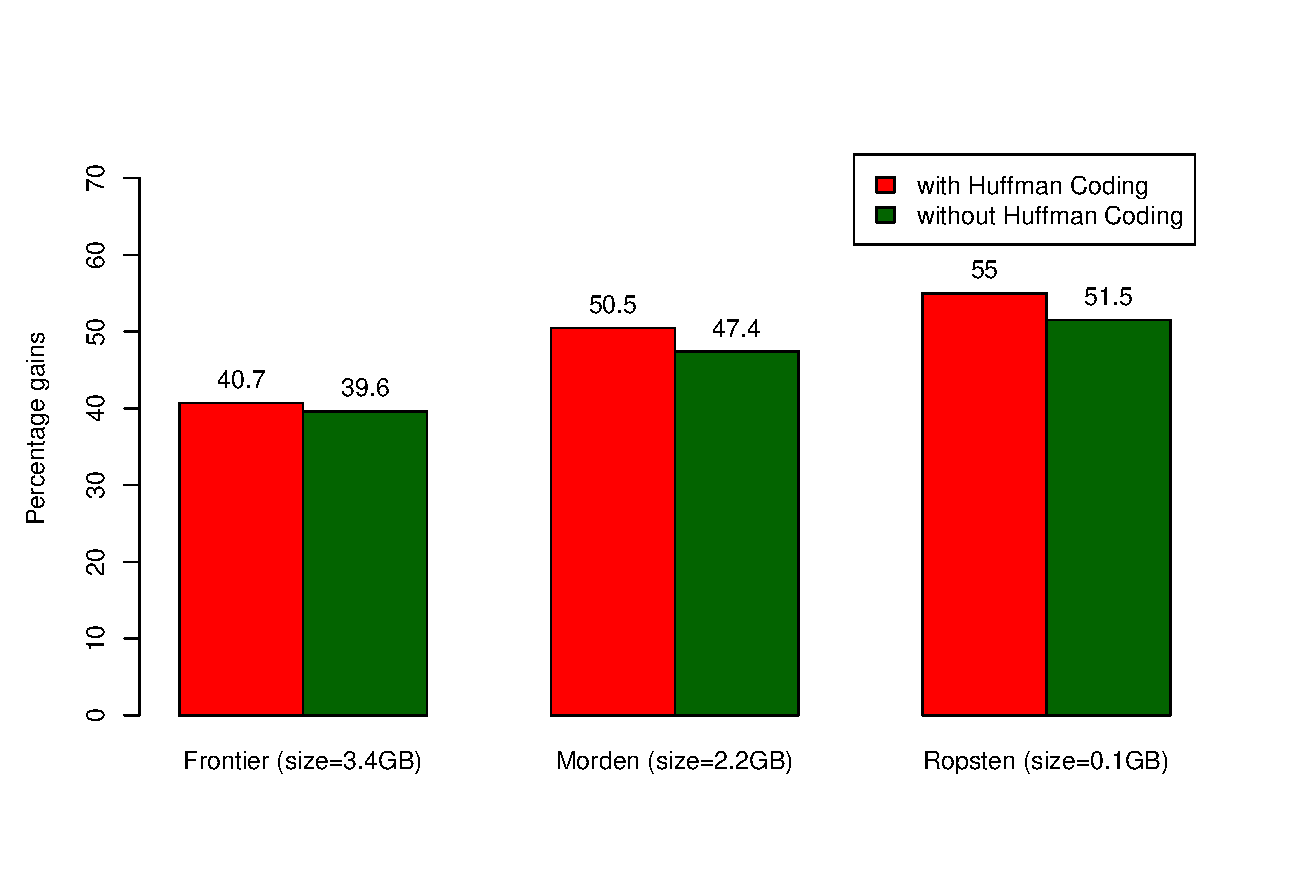
\includegraphics[scale=0.39]{plots/customgains}
	%\rule{3cm}{3cm}
}{ \caption{Percentage gains}
\label{fig:origvscustom}
}
\end{floatrow}
\end{figure}

\FloatBarrier
Table~\ref{tab:origvscustom} shows the size of the blockchains before and after applying our technique. Third and fourth columns show the impact of assigning Huffman codes to EVM opcodes. 
As expected, using Huffman codes lead to further savings because frequently
used opcodes now use fewer bits.
\autoref{fig:origvscustom} shows the percentage gain in space savings due to our technique. This is a standard computation:
\[ 
	\text{percentage gain} = \big ( 1 - \frac{\text{size of custom formatted blockchain}}{\text{size of original blockchain}}\big ) \times 100
\]
Savings are greater when Huffman code are assigned and are as high as $55\%$ for Ropsten. Even on Frontier blockchain, $40\%$ space savings can be observed demonstrating the usefulness of our technique. 
Interestingly, Huffman codes did not bring about lot of savings for Frontier ($\sim1\%$) though they result in about $3\%$ additional savings in Morden and Ropsten networks.
We attribute this to two possibilities:
\begin{enumerate*}
	\item Our Huffman code assignment uses the opcode frequency distribution from Morden network. The Frontier network may have a slightly different distribution.
	\item EVM bytecode constitutes about $13\%$ of the Morden blockchain  but only $8\%$ of the frontier blockchain. 
		This is probably not a huge difference, but could contribute to smaller savings.
\end{enumerate*}

As mentioned earlier, we do not aim to compete against the existing mature compression tools.
However, we provide a comparative evaluation of our tool against gzip, bzip2 and xz. 
These programs are tuned for best compression savings, i.e., \emph{gzip -9}, \emph{bzip2 -9} and \emph{xz -9} have been used. 
Note that the options are only tuned for getting best space savings and may result in increased compression times.
This is a reasonable trade-off given that our primary objective is to get best compression savings in terms of space.
We also evaluate the compression times to ensure that they are not
prohibitively longer.

\begin{table}[H]
\centering
\captionsetup{justification=centering}
\begin{tabular}{ >{\bfseries}c| p{2cm} | p{2cm} |p{2cm} | p{1.5cm} | p{1.5cm} }
	Program & {Compressed Size of Original File (MB)} & {Compressed Size on Custom format (MB)} & {Compressed Size on Custom format with Huffman Encoding (MB)}& Percentage Gain without Huffman Encoding & Percentage Gain with Huffman Encoding\\
  \hline
  gzip  & 33.4 & 27.5 & 29.4 & 17.7 & 12.0 \\
  bzip2 & 31.0 & 26.7 & 28.6 & 13.9 & 7.8  \\
  xz   & 27.8 & 22.4 &  23.3 & 19.4 & 16.2 \\
\end{tabular}
\caption{Compression of Ropsten testnet. \\ Original Size = 98.6MB. Custom format size = 47.8MB}
\label{tab:compropsten}
\end{table}
\autoref{tab:compropsten} 
shows the additional compression savings that were possible by compressing 
our custom format for Ropsten.
First column shows the size of original compressed blockchain 
while
second and third columns show the size after compressing the custom formatted blockchain using gzip, bzip2 and xz. 
As can been, compressing custom format leads to additional $18\%$, $14\%$ and $20\%$ (approximately) gains. Interestingly, all these gains are seen when
Huffman codes are not used. We discuss this later.



\begin{table}[H]
\centering
\captionsetup{justification=centering}
\begin{tabular}{ >{\bfseries}c| p{2cm} | p{2cm} | p{2cm} | p{1.5cm} | p{1.5cm} }
	Program & {Compressed Size of Original File (MB)} & {Compressed Size on Custom format (MB)} & {Compressed Size on Custom format with Huffman Encoding (MB)} & Percentage Gain without Huffman Encoding & Percentage Gain with Huffman Encoding \\
  \hline
  gzip  & 812.2 & 701.3 & 739.6 & 13.7 & 9.0 \\
  bzip2 & 762.9 & 685.6 & 725.8 & 10.1 & 5.0 \\
  xz   & 686.7 & 599.2 &  620.7 & 12.7 & 9.6 \\
\end{tabular}
\caption{Compression of Morden testnet. \\Original Size = 2160MB. Custom format size = 1135.4MB}
\label{tab:compmorden}
\end{table}
\autoref{tab:compmorden} 
shows the additional compression savings that were possible by compressing 
our custom format for Morden using gzip, bzip2 and xz.
As can been, compressing custom format leads to additional $14\%$, $10\%$ and $13\%$  gains. Again, all these gains are seen when Huffman codes are not used. 

\begin{table}[H]
	\centering
\captionsetup{justification=centering}
\begin{tabular}{ >{\bfseries}c| p{2cm} | p{2cm} | p{2cm} | p{1.5cm} | p{1.5cm} }
	Program & {Compressed Size of Original File (MB)} & {Compressed Size on Custom format without Huffman Encoding (MB)} & {Compressed Size on Custom format with Huffman Encoding (MB)} &Percentage Gain without Huffman Encoding & Percentage Gain with Huffman Encoding\\
  \hline
  gzip  & 1807.1 & 1481.1 & 1627.9 & 18.0 & 10.1 \\
  bzip2 & 1751.3 & 1474.6 & 1590.0 & 15.8 & 9.2 \\
  xz   & 1541.8 & 1367.6 & 1398.7 & 11.3  & 9.3 \\
\end{tabular}
\caption{Compression of Frontier mainnet. \\ Original Size = 3434.6MB. Custom format size = 2069MB}
\label{tab:compfrontier}
\end{table}
\autoref{tab:compfrontier} 
shows the additional compression savings that were possible by compressing 
our custom format for Frontier  using gzip, bzip2 and xz.
As can been, compressing custom format leads to additional $18\%$, $16\%$ and $11\%$  gains. Again, all these gains are seen when
Huffman codes are not used. It is worth noting that this blockchain
is the actual \eth{} blockchain and the gains are therefore real.
Using xz and our custom format, we are able to
bring down the size of the blockchain from 3.3GB to 1.4GB, 
resulting in about $58\%$ space savings.
As the blockchain grows on the orders of giga bytes, these savings are significant.
In all the above cases above, xz has the best compression performance on the original blockchain. 
Our custom format enables further improvement ($10-20\%$) even in the best case.

\begin{figure}[H]
	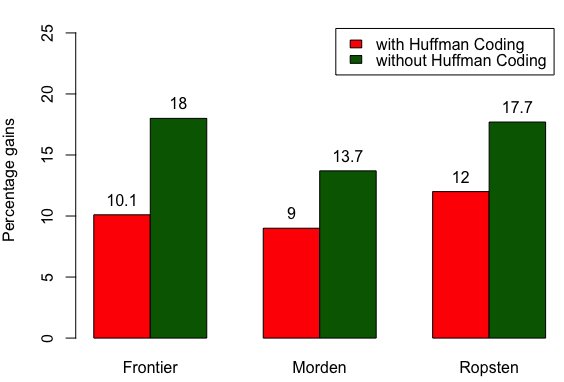
\includegraphics[scale=0.45]{plots/gzip}
	\caption{Additional compression gains (\%) using gzip}
	\label{fig:gzip}
\end{figure}

\begin{figure}[H]
\begin{subfigure}{0.45\textwidth}
	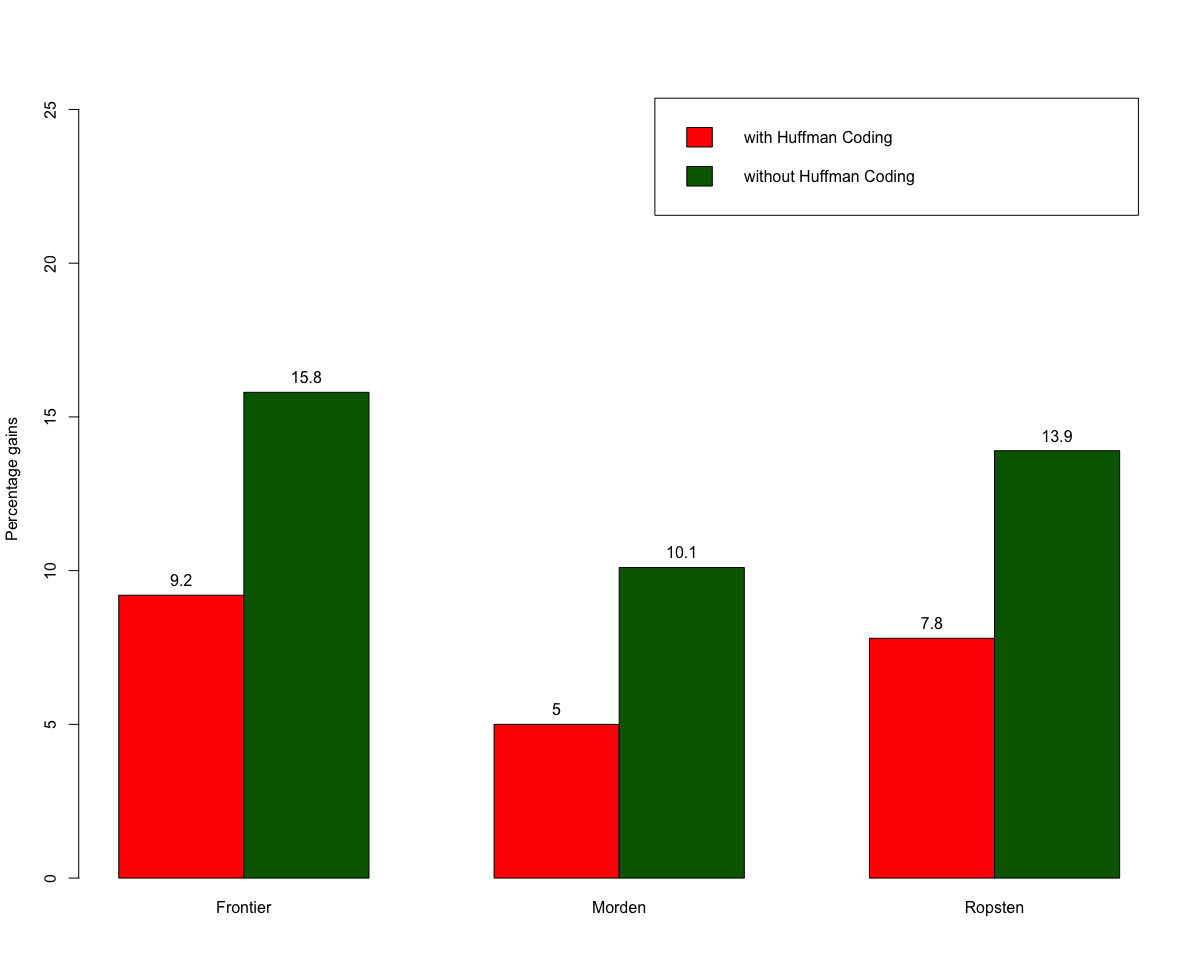
\includegraphics[width=\textwidth]{plots/bzip2-vanilla}
	\caption{Additional compression gains (\%) using bzip2}
	\label{fig:bzip2}
\end{subfigure}
\begin{subfigure}{0.45\textwidth}
	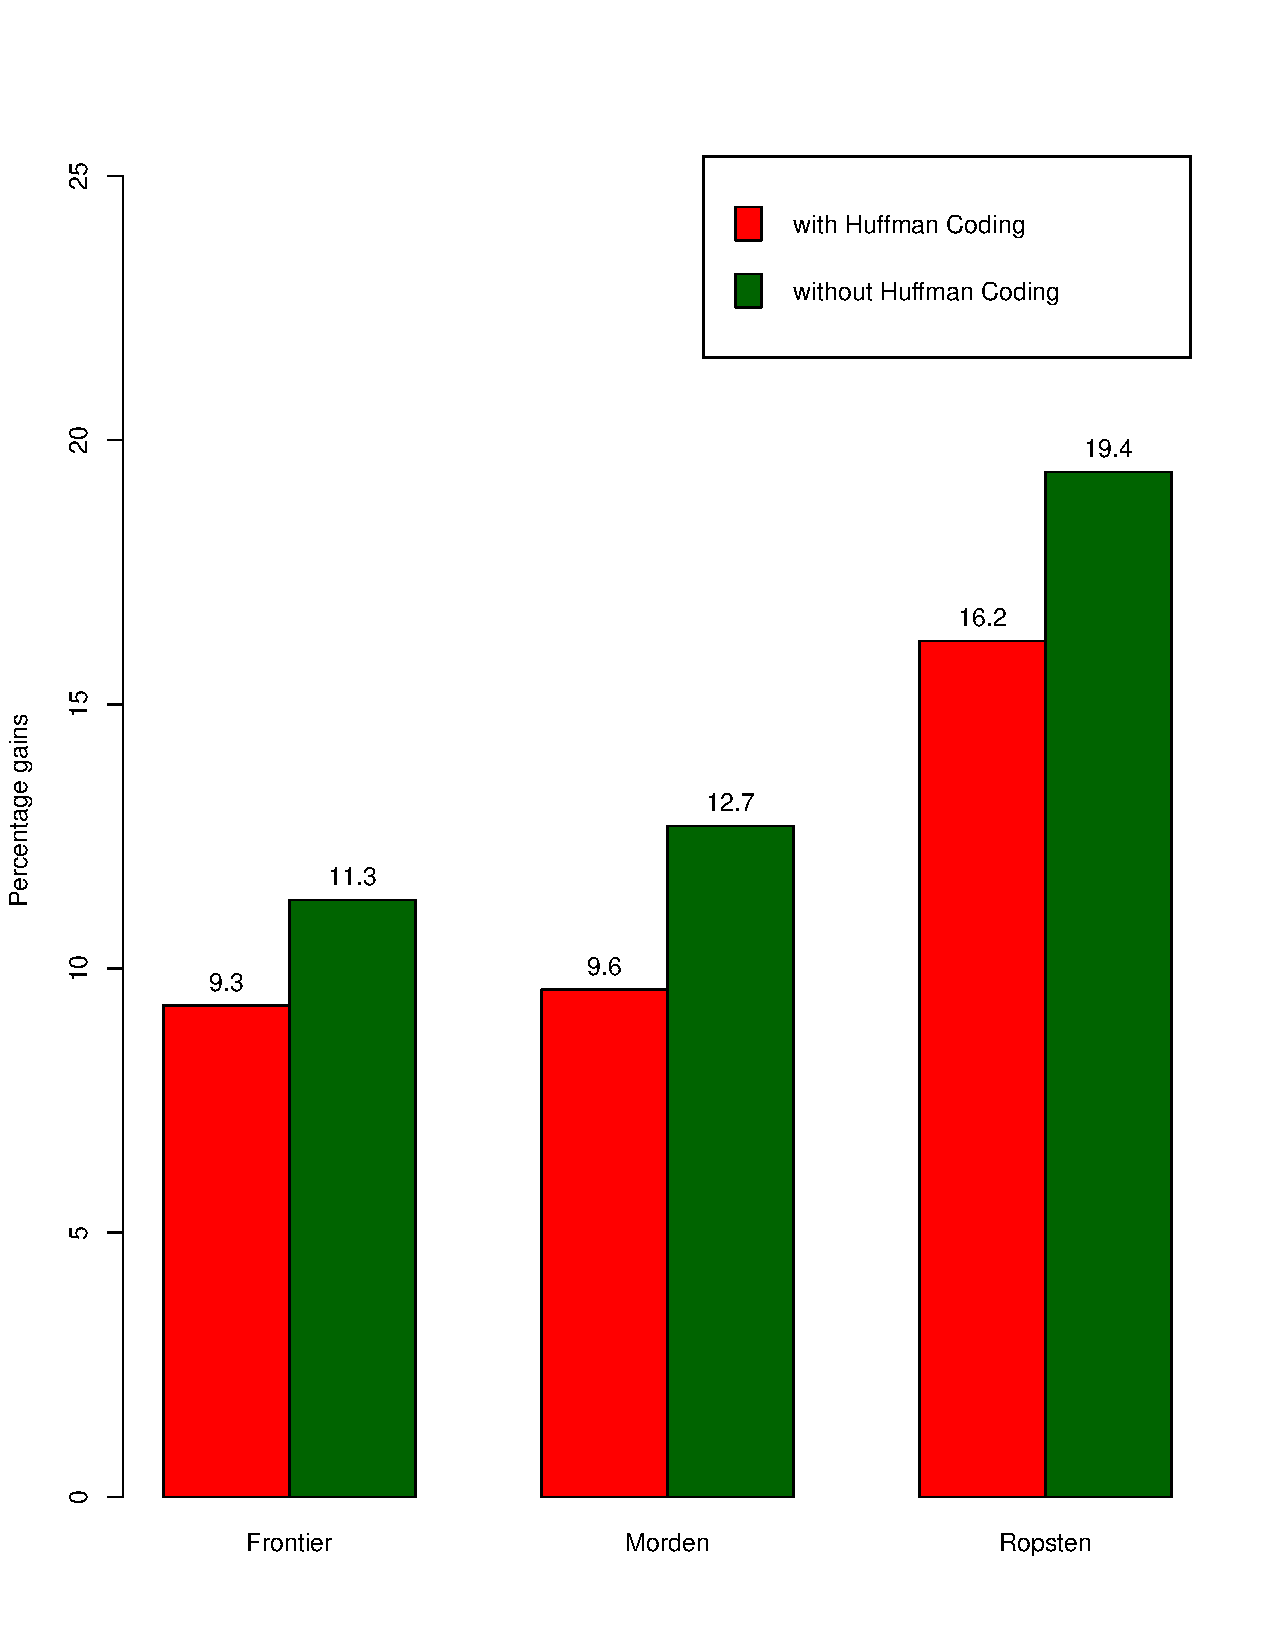
\includegraphics[width=\textwidth]{plots/xz-vanilla}
	\caption{Additional compression gains (\%) using xz}
	\label{fig:xz}
\end{subfigure}
\caption{ }
\end{figure}
We summarize the additional compression gains for each compression scheme in \autoref{fig:gzip}, \autoref{fig:bzip2} and \autoref{fig:xz}.
As we can see, the results are encouraging and show room for improvement upto $20\%$ (Ropsten in xz).

To demonstrate the feasibility of our approach, we also measure the time taken for compression. 
For brevity, we only present the values for compressing Morden blockchain.
The runtime performance of our tool is proportional to the total number of blocks and transactions. 
To generate the custom format without Huffman encoding, it takes about 150 seconds to generate the custom format and with Huffman encoding it takes about 250 seconds. 



\begin{table}[H]
	\centering
	\begin{tabular}{>{\bfseries}c | p{3cm} | p{3cm}} 
	Program & {Original Compression Time} & {Compression Time using our custom format} \\
	\hline
	gzip & 220  & 71 \\
	bzip2 & 360  & 245\\
	xz & 1340 & 520 \\
	\end{tabular}
	\caption{Compression time in seconds}
	\label{tab:comptime}
\end{table}
\autoref{tab:comptime} compares the time taken to compress the binaries before and after applying our technique. As expected, it is less for binaries that are in custom format. 
To make a fair comparison, we should also include the time taken to create the custom format i.e., 150 and 250 seconds depending on whether Huffman encoding is turned on.
It is worth noting that our tool is a prototype and is not optimized for runtime performance. 
Yet, the performance is comparable. 
In fact, it outperforms in the case of xz which is encouraging.
\begin{figure}[H]
	\centering
	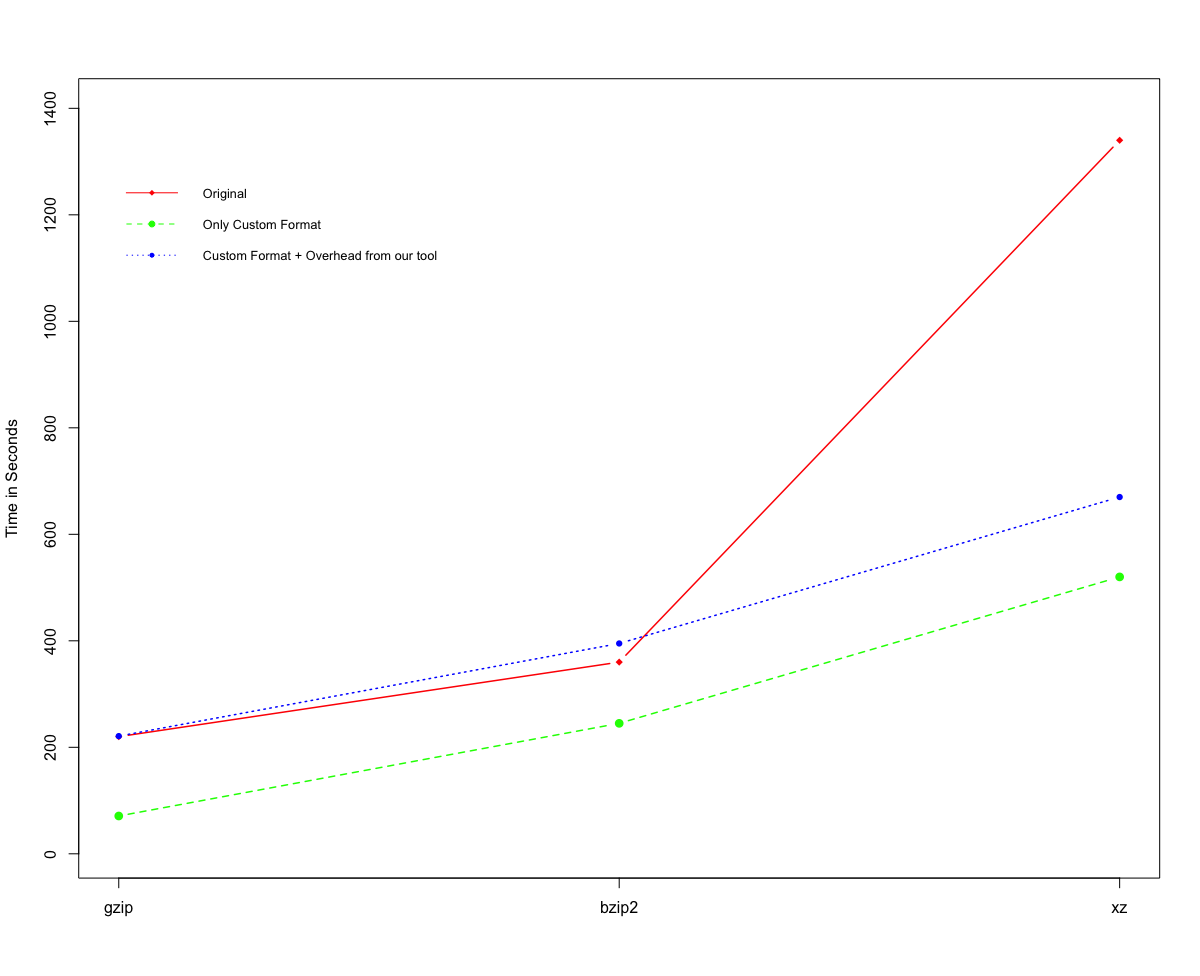
\includegraphics[width=0.5\textwidth, scale=0.5]{plots/time}
	\caption{Compression time in seconds}
	\label{fig:comptime}
\end{figure}
\autoref{fig:comptime} shows the compression time for the original and custom formatted blockchains using gzip, bzip2 and xz.
The dotted green and blue lines show the compression with and without our tool
overheads. In case of xz the total compression time (including the overhead) is about half the original one.

